\documentclass[a4paper]{article}
\usepackage[utf8]{inputenc}
\usepackage[spanish, es-tabla, es-noshorthands]{babel}
\usepackage[table,xcdraw]{xcolor}
\usepackage[a4paper, footnotesep = 1cm, width=22cm, top=2.5cm, height=25cm, textwidth=20cm, textheight=25cm]{geometry}
%\geometry{showframe}

\usepackage{tikz}
\usepackage{amsmath}
\usepackage{amsfonts}
\usepackage{amssymb}
\usepackage{float}
\usepackage{graphicx}
\usepackage{caption}
\usepackage{subcaption}
\usepackage{multicol}
\usepackage{multirow}
\usepackage{wrapfig}
\setlength{\doublerulesep}{\arrayrulewidth}
\usepackage{booktabs}

\usepackage{hyperref}
\hypersetup{
    colorlinks=true,
    linkcolor=blue,
    filecolor=magenta,      
    urlcolor=blue,
    citecolor=blue,    
}

\newcommand{\note}[1]{
	\begin{center}
		\huge{ \textcolor{red}{#1} }
	\end{center}
}

\setcounter{topnumber}{2}
\setcounter{bottomnumber}{2}
\setcounter{totalnumber}{4}
\renewcommand{\topfraction}{0.85}
\renewcommand{\bottomfraction}{0.85}
\renewcommand{\textfraction}{0.15}
\renewcommand{\floatpagefraction}{0.8}
\renewcommand{\textfraction}{0.1}
\setlength{\floatsep}{5pt plus 2pt minus 2pt}
\setlength{\textfloatsep}{5pt plus 2pt minus 2pt}
\setlength{\intextsep}{5pt plus 2pt minus 2pt}

\newcommand{\quotes}[1]{``#1''}
\usepackage{array}
\newcolumntype{C}[1]{>{\centering\let\newline\\\arraybackslash\hspace{0pt}}m{#1}}
\usepackage[american]{circuitikz}
\usetikzlibrary{calc}
\usepackage{fancyhdr}
\usepackage{units} 

\graphicspath{{../Ejercicio-1/}{../Ejercicio-2/}{../Ejercicio-3/}{../Ejercicio-4/}}

\pagestyle{fancy}
\fancyhf{}
\lhead{31.99 -  Mecatrónica Aplicada}
\rhead{Lambertucci}
\rfoot{Página \thepage}


\begin{document}

%%%%%%%%%%%%%%%%%%%%%%%%%
%		Caratula		%
%%%%%%%%%%%%%%%%%%%%%%%%%

\begin{titlepage}
\newcommand{\HRule}{\rule{\linewidth}{0.5mm}}
\center
\mbox{\textsc{\LARGE \bfseries {Instituto Tecnológico de Buenos Aires}}}\\[1.5cm]
\textsc{\Large 31.99 -  Mecatrónica Aplicada}\\[0.5cm]


\HRule \\[0.6cm]
{ \Huge \bfseries Trabajo práctico N$^{\circ}$I}\\[0.4cm] 
{\huge One Wheel}\\
\HRule \\[1.5cm]


{\large

\emph{Alumno}\\
\vspace{3px}

\begin{tabular}{lr} 	
\textsc{Lambertucci}, Guido Enrique  & 58009 \\
\end{tabular}

\vspace{20px}

\emph{Profesores}\\

\textsc{Perfumo}, Lucas Alberto\\
\textsc{Basualdo}, Hernán Federico\\




\vspace{3px}
%\textsc{} \\	

\vspace{100px}

\begin{tabular}{ll}

Presentado: & 18/08/21\\

\end{tabular}

}

\vfill

\end{titlepage}


%%%%%%%%%%%%%%%%%%%%%
%		Indice		%
%%%%%%%%%%%%%%%%%%%%%

\tableofcontents
\newpage

%%%%%%%%%%%%%%%%%%%%%
%		Informe		%
%%%%%%%%%%%%%%%%%%%%%


\section{Introducci\'on}

En el siguiente trabajo de ingenier\'ia inversa se eligi\'o como producto el One Wheel.
Es una patineta el\'ectrica usada mayormente con fines recreativos,aunque tambi\'en es utilizada para transporte.
%Describan el proyecto en forma general y sintética (uso, función, finalidad, etc). Campos de aplicación y antecedentes.
\begin{figure}[H]
	\center
	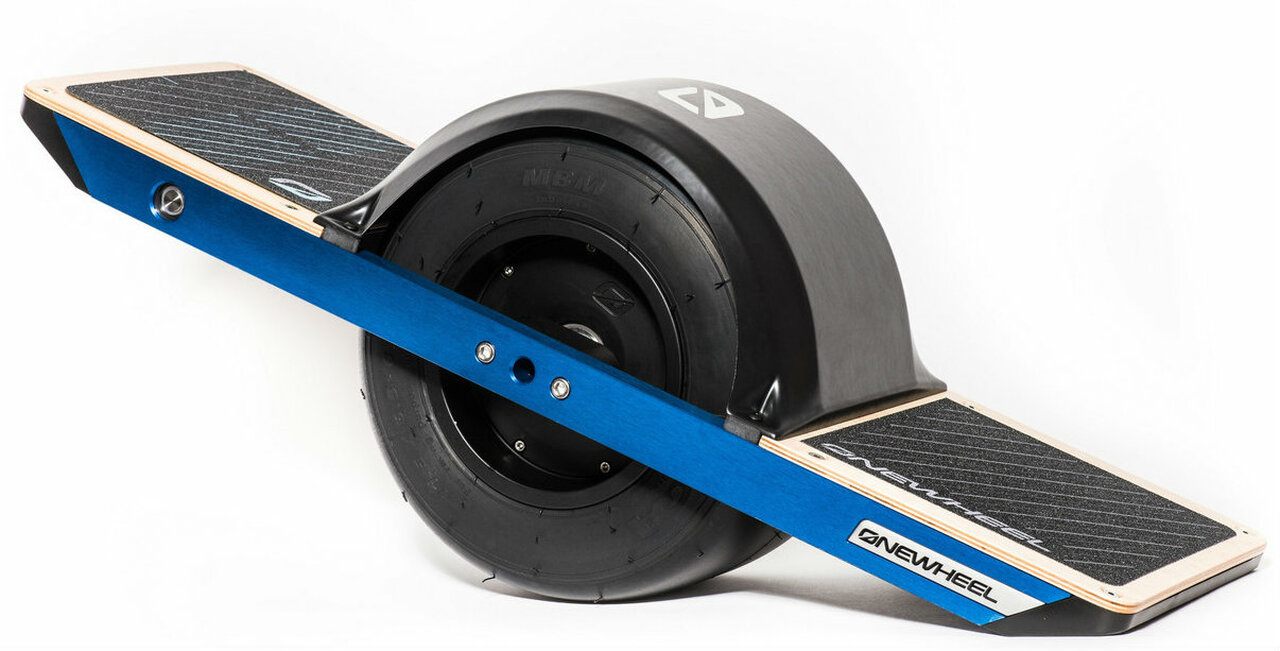
\includegraphics[width=0.6\linewidth, page=1]{Imagenes/onewheel}
	\caption{OneWheel.}
	\label{fig:intro:OneWheel}
\end{figure}
\subsection{Uso}
Para su uso basta con colocar los pies sobre las superficies con lija e impulsarse para poner la patineta en posición horizontal. Esto activar\'a el sistema de balance autom\'atico de la patineta, el cual equilibrar\'a la tabla en posci\'on horizontal. Para acelerar basta con desplazar el peso de uno en la dirección deseada, lo cual indicar\'a a la tabla el cambio que debe hacer.
\subsection{Alternativas}
En el mercado existe otras alternativas similares al OneWheel tales como el monociclo eléctrico.
 \begin{figure}[H]
	\center
	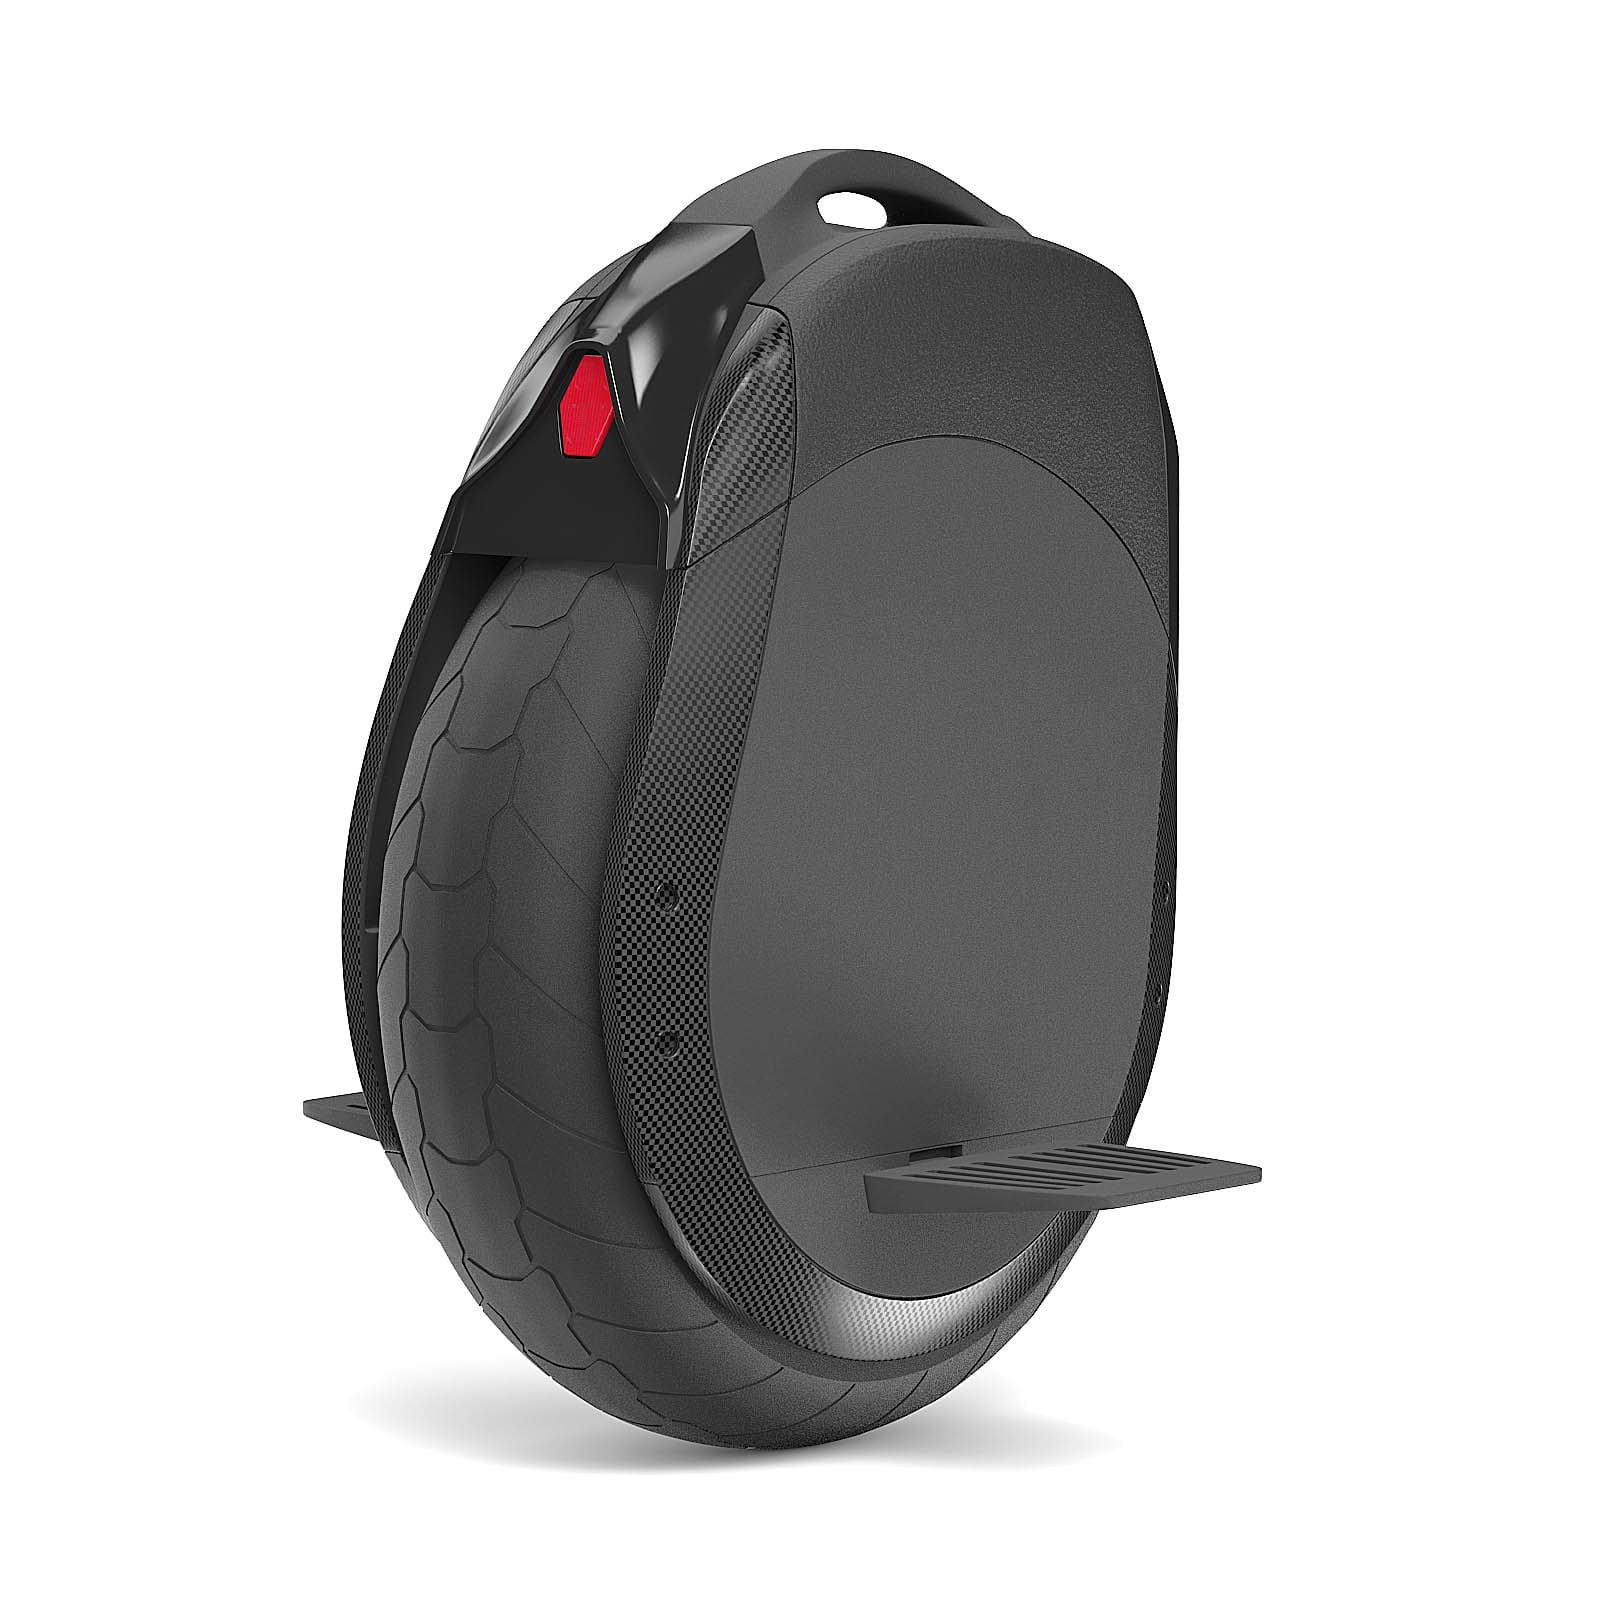
\includegraphics[width=0.4\linewidth, page=1]{Imagenes/antescedentes}
	\caption{Monociclo el\'ectrico.}
	\label{fig:intro:monociclo_electrico}
\end{figure}
Algunas características en las que difieren estas dos alternativas son: la posici\'on en la que uno pone las piernas, la direcci\'on de avance (con los pies ortogonales al movimiento o no)
el tamaño y el perfil de uso.
\section{Esquema f\'isico}
El OneWheel está compuesto por diversas partes dentro de ellas se pueden mencionar los siguientes elementos
 \begin{figure}[H]
	\center
	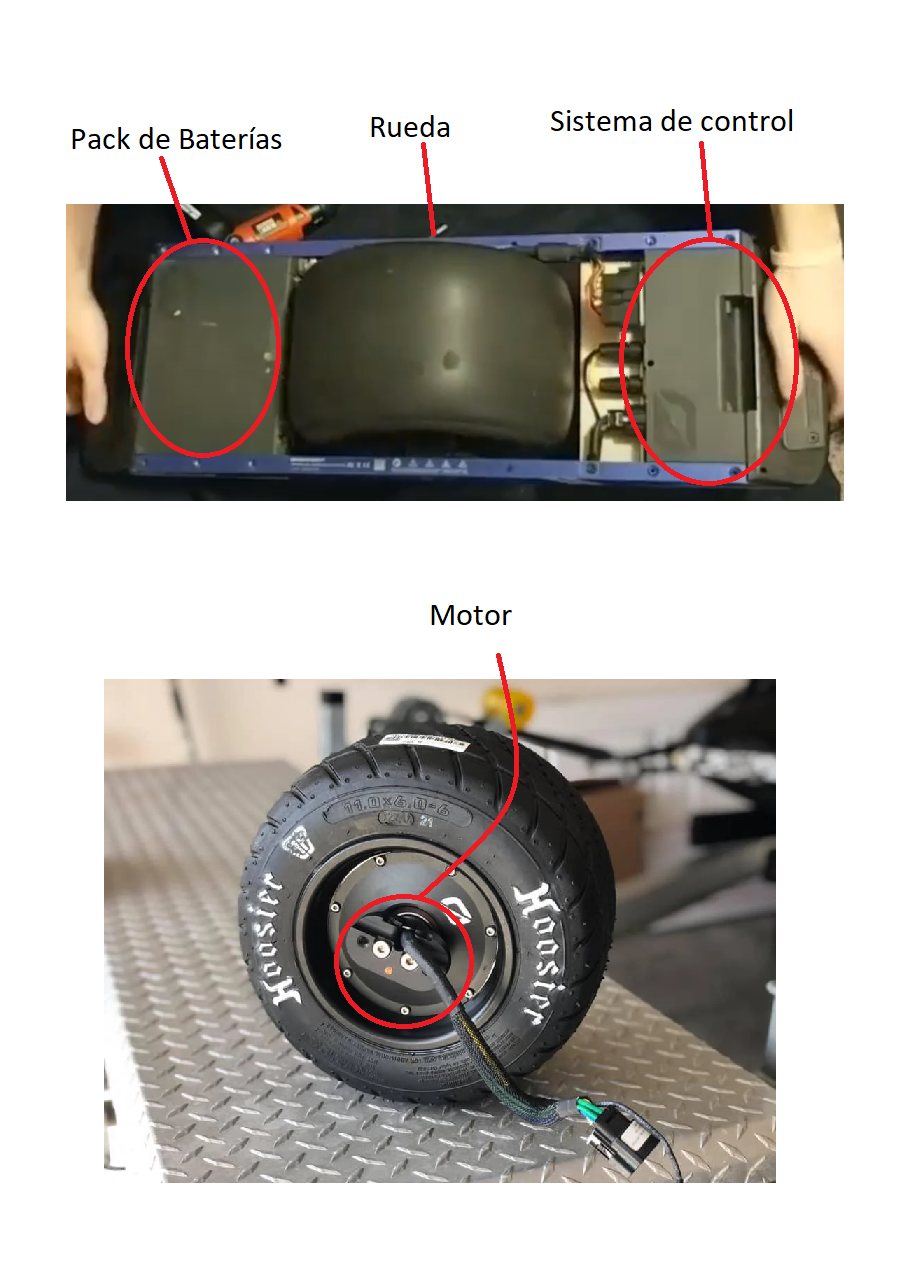
\includegraphics[width=0.4\linewidth, page=1]{Imagenes/Diagrama}
	\caption{Esquema de componentes.}
	\label{fig:Esq_fisico:diagrama}
\end{figure}
Ademas en la unidad de control se distinguen una unidad de medidas inerciales (IMU), algún microcontrolador (MCU) para realizar el control programable, baterías, rueda, una carcasa con antideslizantes. 



%Su función global, funcionamiento y sus partes constitutivas (Descriptivo y sintético); pueden resolver a mano alzada o capturando imágenes representativas.

\section{Esquema de control}
\subsection{Variable de medici\'on}
Las variables de medición son el ángulo respecto de la normal a la tierra. Ya que en el sistema de control de balance automático tiene como finalidad mantener el ángulo ortogonal al piso, el control de velocidad es realizado por otro sistema.
  
\subsection{Sensores}
Los sensores utilizados en el sistema de balance automático del OneWheel son:
\begin{itemize}
\item Aceler\'ometro
\item Magnetómetro
\item Giróscopo
\end{itemize}
\subsubsection{Aceler\'ometro}
El aceler\'ometro como su nombre indica mide la magnitud f\'isica de la aceleraci\'on, el principio de funcionamiento del utilizado en el OneWheel consiste en la medici\'on de una capacidad que resulta proporcional a la aceleraci\'on.


Esto se debe a como est\'a diseñado el sensor. Cuenta con una masa unida a unos resortes, esta masa tiene unas paletas a lo largo de su cuerpo, que se intercalan con otras ajenas a la masa. Cuando esta masa sufre una aceleraci\'on , la distancia entre las paletas de la masa y las ajenas a la misma cambian, por lo tanto la capacidad entre ellas var\'ia. 
 \begin{figure}[H]
	\center
	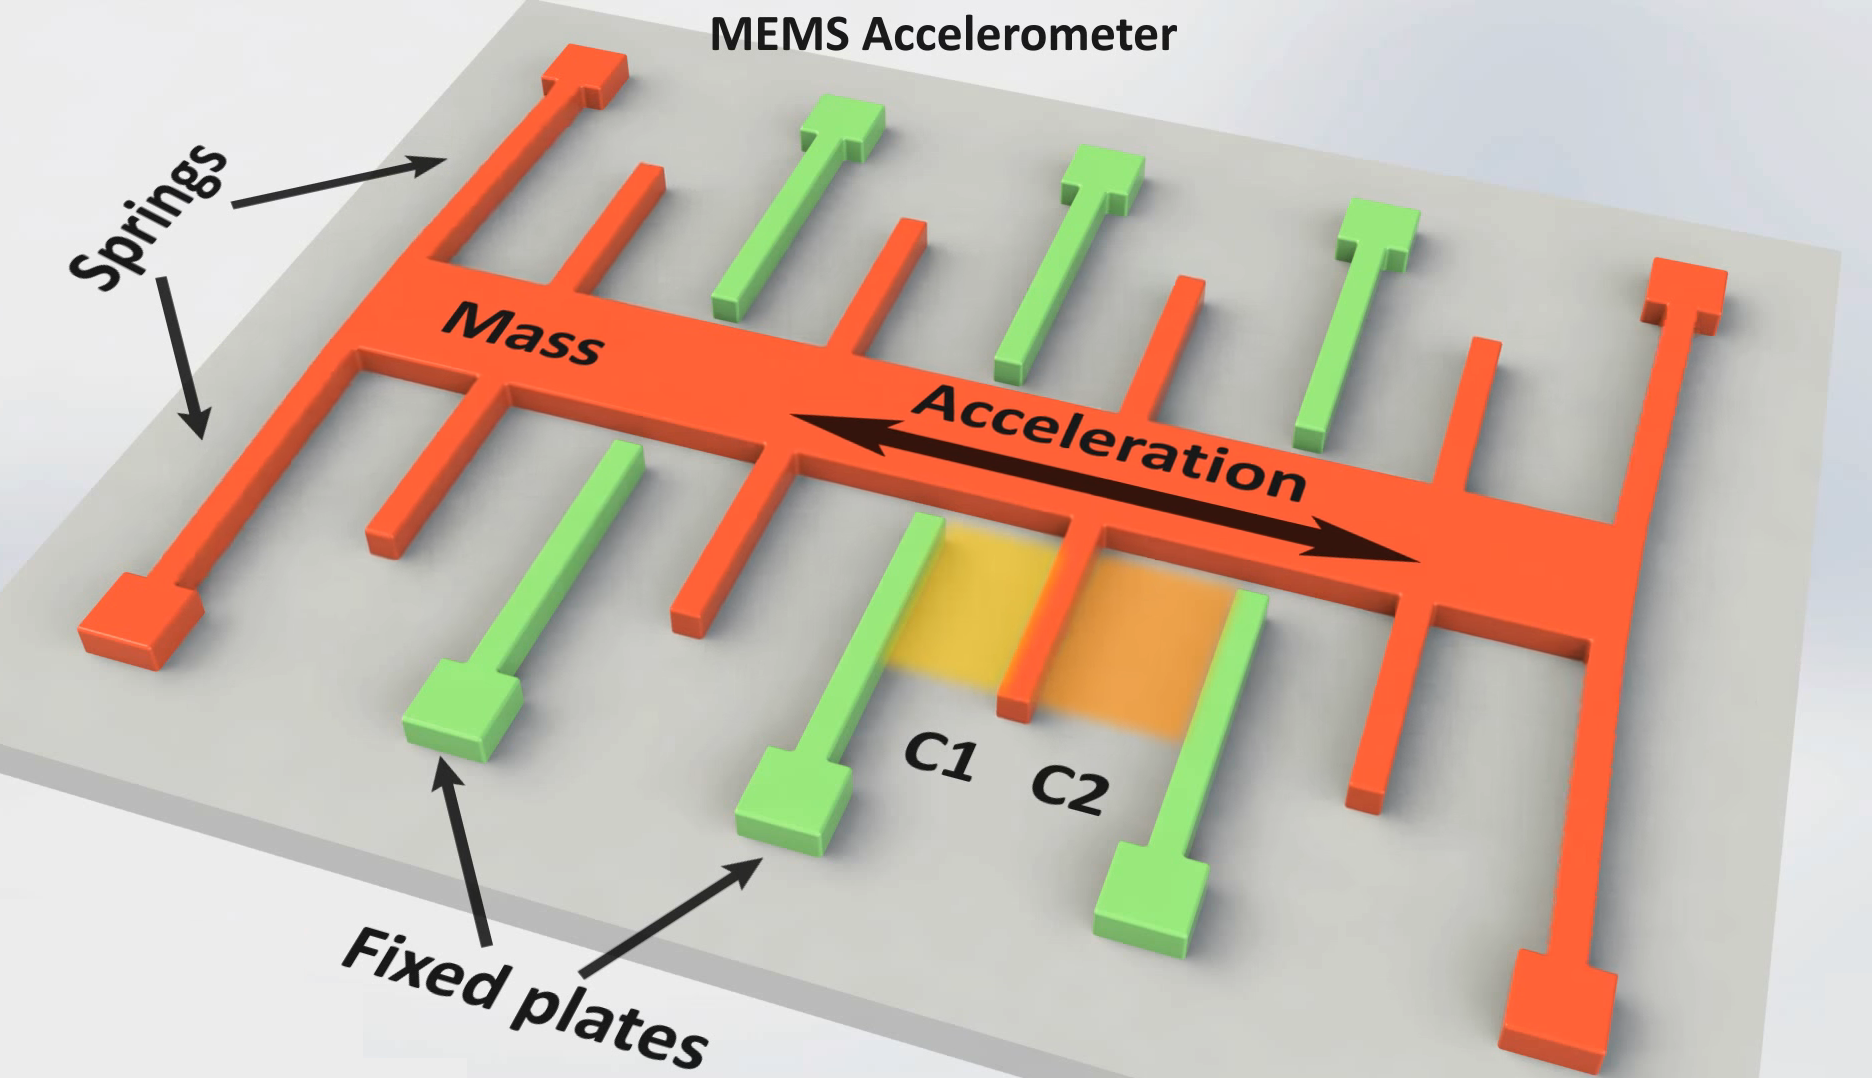
\includegraphics[width=0.5\linewidth, page=1]{Imagenes/accelerometer}
	\caption{Aceler\'ometro.}
	\label{fig:Esq_con:acelerometro}
\end{figure}
Este esquema es \'util para ilustrar el principio de funcionamiento del aceler\'ometro, aunque vale la pena mencionar que este esquema permite medir la aceleraci\'on en un solo eje. Deber\'ian utilizarse 3 de estos dispositvos para poder medir los 3 ejes.
\subsubsection{Giróscopo}
El gir\'oscopo mided velocidad angular utilizando el efecto coreolis. El efecto coreolis enuncia que:
\begin{equation}
\vec{F_c} = -2m \left( \vec{\omega} \times \vec{v} \right)
\label{eq:coreolis}
\end{equation}
Como se observa en la ecuaci\'on (\ref{eq:coreolis}) para que haya efecto coreolis debe haber una velocidad no nula. Por lo que la microestructura del sensor es la siguiente:
Hay una masa (rojo) la cual se encuentra en movimiento constante (debido a la masa amarilla), la masa roja tiene un sistema similar al del aceler\'ometro, donde cambia la capacidad dependiendo la posici\'on, cuando al sistema se le agrega una velocidad angular a la masa se le agrega una componente ortogonal en su movimiento (debido a la fuerza coreolis) por o que cambiara la capacidad entre las paletas y se podr\'a obtener la velocidad angular. 
 \begin{figure}[H]
	\center
	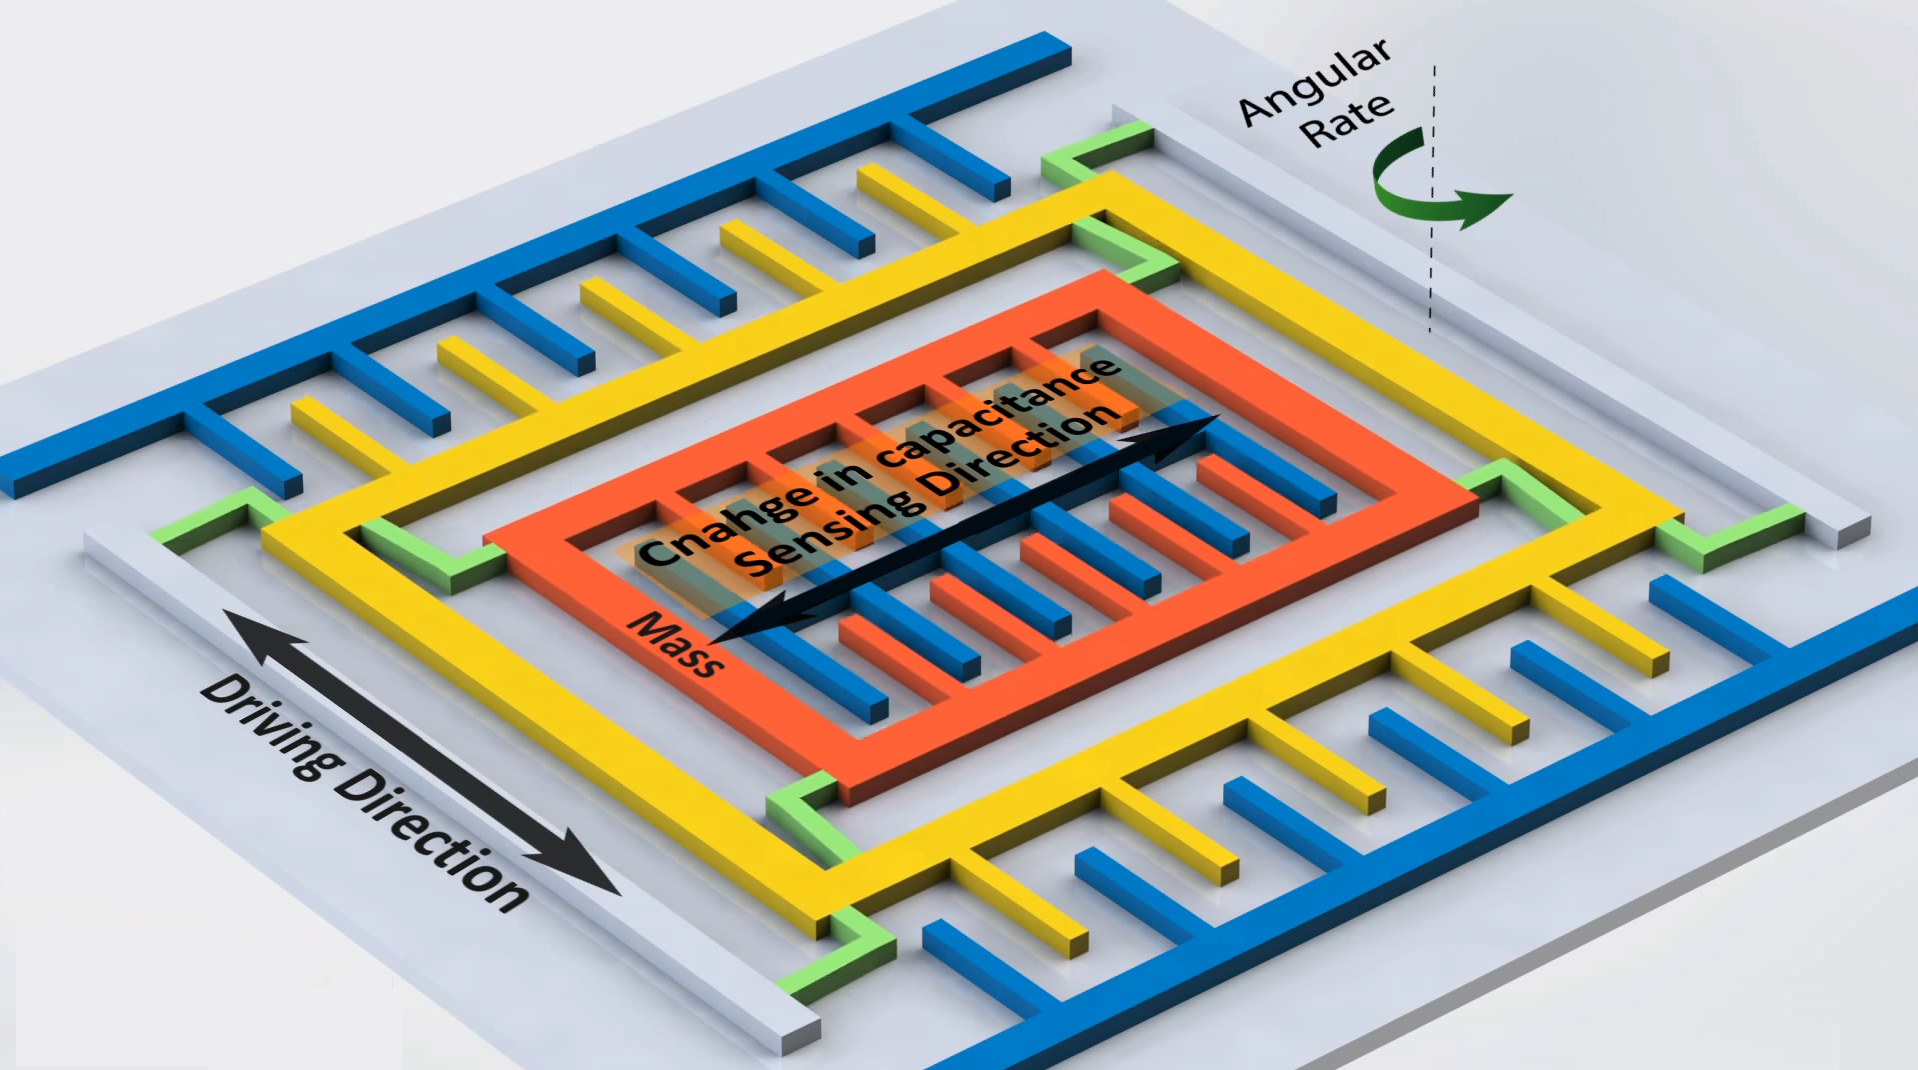
\includegraphics[width=0.5\linewidth, page=1]{Imagenes/giroscopo}
	\caption{Gir\'oscopo.}
	\label{fig:Esq_con:giroscopo}
\end{figure}
Al igual que el aceler\'ometro esto permite la medici\'on en un eje, y para obtener los otros se necesitar\'an mas sensores.
\subsubsection{Magnetómetro}  
En cuanto a los magnet\'ometros pueden existir en dos tecnolog\'ias usualmente, los que utilizan el efecto Hall y los que usan el efecto magneto-resistivo ambos con el fin de medir el campo magnetico $\vec{H}$.


El efecto Hall dice que dada una corriente que esta circulando por un conductor, al acercar un campo magnético este polarizar\'a el material, pudiendo medir una diferencia de potencial entre los extremos del conductor, proporcional al campo magnético. El efecto magnetoresistivo se basa en utilizar elementos cuya resistencia sea sensible a campos magn\'eticos tales como el hierro y el n\'iquel
 \begin{figure}[H]
	\center
	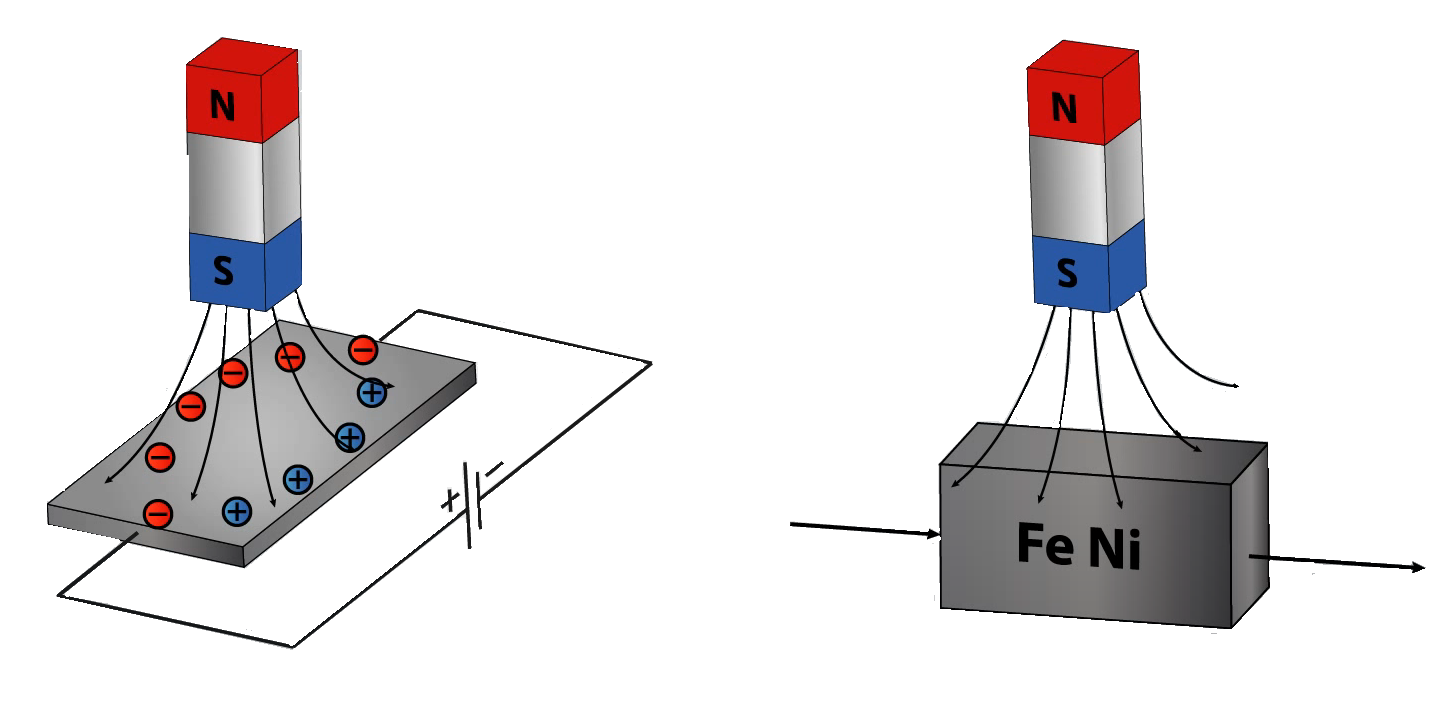
\includegraphics[width=0.5\linewidth, page=1]{Imagenes/magnetometro}
	\caption{Magnet\'ometro.}
	\label{fig:Esq_con:magnetometro}
\end{figure}

\subsubsection{Sensor fusion}
La t\'ecnica de \textit{sensor fusion} consiste en combinar las mediciones de por lo menos 2 fuentes de informaci\'on en una manera que genere un \textbf{mejor entendimiento} del sistema estudiado. Donde por mejor entendimiento se interpreta como mas consistente, mas preciso, mas confiable.


En el caso del OneWheel vamos a utilizar sensor fusion para estimar la rotación de la tabla respecto de la normal de la tierra. Para esto se elige como marco de referencia de la tierra, los puntos cardinales norte y este, y la dirección "Abajo". Para ubicar la posición de la tabla en función del marco de refernecia mencionado basta con utilizar el acelerómetro y el magnetómetro. Si se asume que la tabla se encuentra estática se puede medir la aceleración la cual indicará que dirección es arriba (opuesta a la gravedad),  luego uno pensaría que para determinar el norte basta con medir la dirección del campo magnético, pero esto no es asi, debido a que las lineas de campo tienen diversos ángulos de ataque dependiendo en que zona del mundo uno se encuentra (Esto no sucede en una brújula debido a que esta se encuentra limitada a un espacio bidimensional).
 \begin{figure}[H]
	\center
	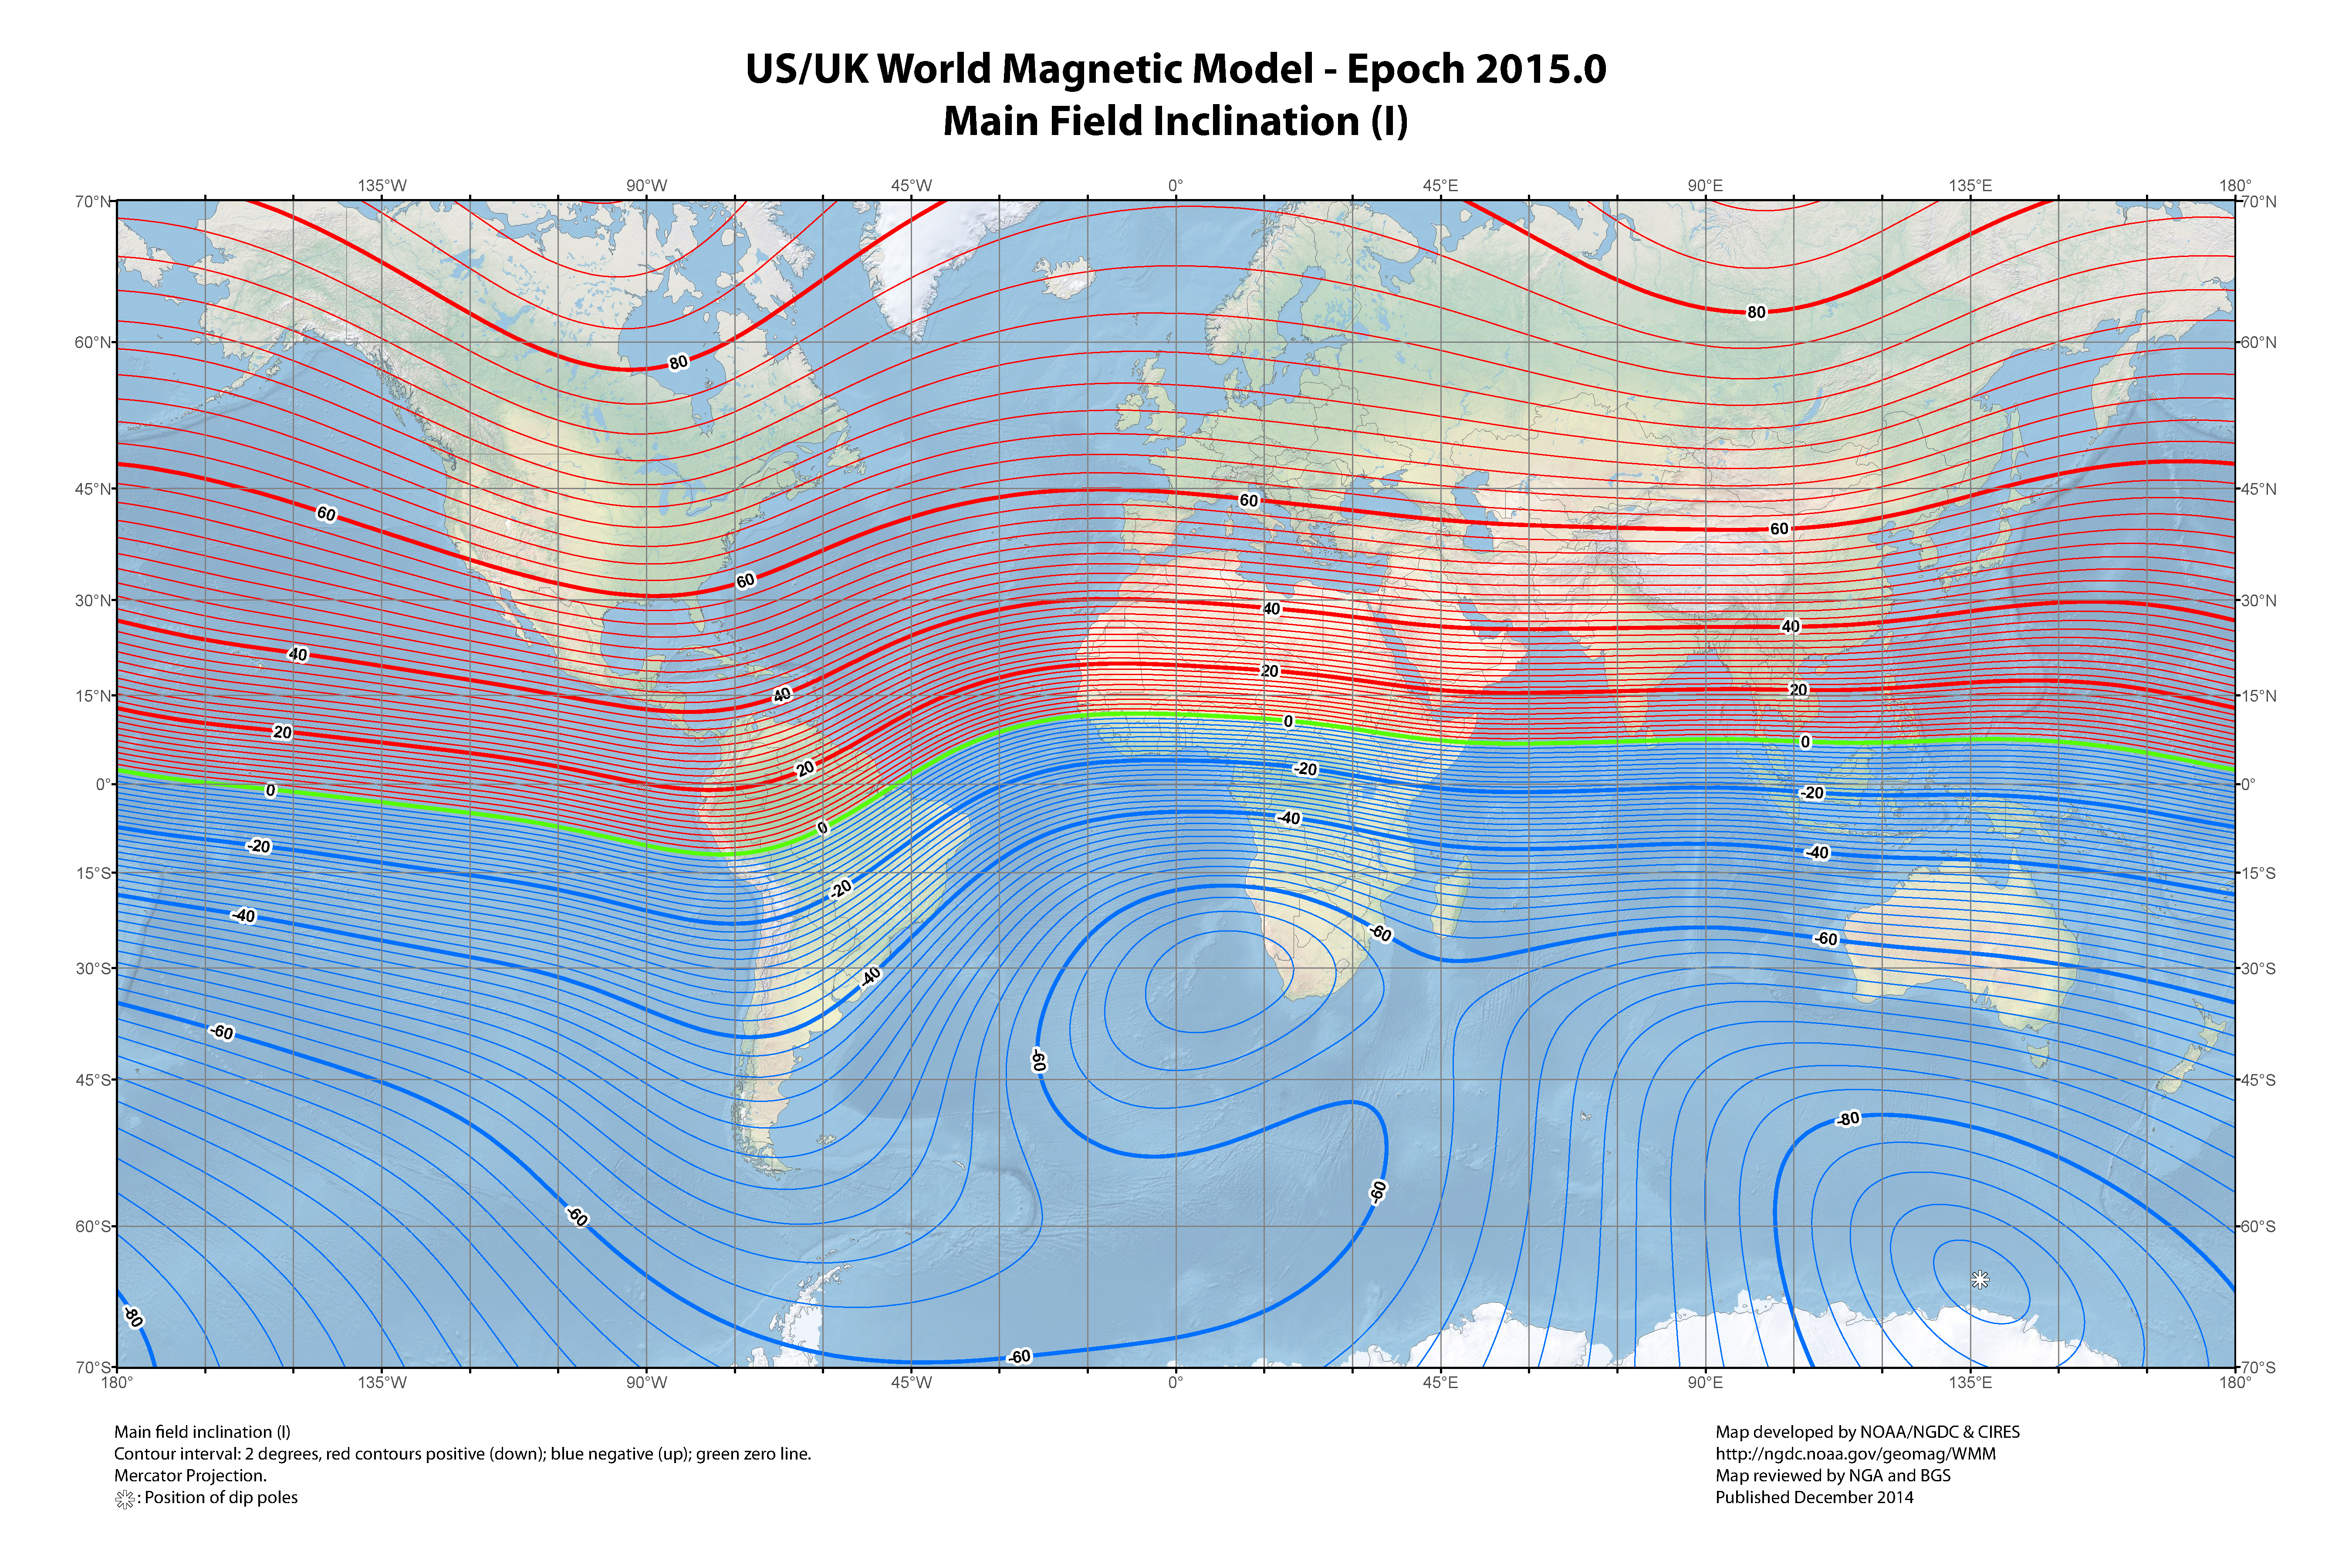
\includegraphics[width=1\linewidth, page=1,]{Imagenes/campo_terrestre}
	\caption{Campo magnético terrestre.}
	\label{fig:Esq_con:campo_terrestre}
\end{figure}
En Argentina por ejemplo este ángulo varía entre -20 y -55 grados. Por lo que el vector claramente no estará únicamente en el sentido norte.

Para obtener el sentido norte basta con realizar productos vectoriales dado que:
\begin{equation}
\vec{Este} \ = \ \vec{Arriba} \  \times \ \vec{H}
\end{equation}
y finalmente 
\begin{equation}
\vec{Norte} \ = \ \vec{Este} \  \times \ \vec{Abajo}
\end{equation}
Queda definido tanto el marco de referencia propio como así también el terrestre. Con ellos se pueden armar los cosenos directores y tener la orientación de la tabla en el espacio.



Si bien esto resulta muy satisfactorio para las condiciones iniciales propuestas, cuando uno mueve la tabla, el acelerómetro no medirá únicamente la aceleración de la gravedad sino que todo tipo de aceleración por lo que no medirá correctamente que dirección es "Abajo". Otro problema que surge depende de donde está ubicado la IMU, dado a que si el acelerómetro no está en el eje de rotación, al rotar detectará una aceleración. 


Otro problema existe debido a que el campo magnético terrestre no es el único que interacciona con el magnetómetro, por lo que la medición no será correcta. Para solucionar este problema hay diversos métodos, si la perturbación magnetica  es parte del sistema y rota con el magnetómetro puede ser calibrado.
Este tipo de perturbaciones se llaman "Hard iron source" y "Soft iron source".


Una "Hard iron source" es una que genera su propio campo magnético, por ejemplo un iman, una bobina, etc. por lo que agrega un campo magnetico fijo ademas del terrestre.


Mientras que una "Soft iron source" es un material ferromagnético  que tendrá el efecto de doblar las lineas de campo magnético.


Estos tipos de perturbaciones tienen distintos efectos en las mediciones del campo, idealmente al rotar e magnetómetro en todas las direcciones, se registraría una esfera centrada en el campo magnetico terrestre, mientras que la contribución de las "Hard iron source" provocarán un offset en el centro de esta esfera, y las "Soft iron source" provocarán una distorsión en esta esfera tornandola en un elipsoide.

 \begin{figure}[H]
	\center
	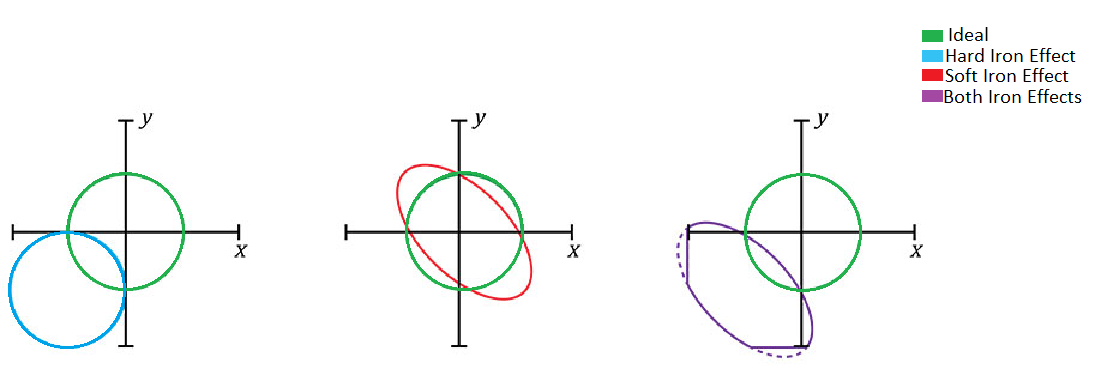
\includegraphics[width=0.8\linewidth, page=1,]{Imagenes/efectos}
	\caption{Campo magnético perturbados.}
	\label{fig:Esq_con:efectos}
\end{figure}
Si se mide el elipsoide desplazado antes de realizar mediciones, se puede encontrar el vector de offset y la matriz de tranformaci\'on que corrige el elipsoide a una esfera perfecta.
\begin{equation}
\vec{x}_{corrected} = (\vec{x}_{meas}-\vec{b}_{off}) \cdot \vec{A} 
\end{equation}

En cuanto al problema de la aceleración plantearemos 2 métodos que pueden trabajar en conjunto para solucionarlo.
El primer método es útil si la aceleración es resultado de los actuadores del sistema. Teniendo un buen modelo del sistema, se puede utilizar un observador de estados para predecir cual será la salida del sistema dado el comando del actuador, y restar la aceleración estimada de la medida, para obtener al gravitatoria.


Si no es posible predecir la aceleración porque esta viene de un sistema ajeno al nuestro, una técnica útil es descartar las mediciones que esten fuera de un rango de 1 \textbf{g} 
\subsection{Actuadores}
\subsubsection{Motores}
\subsection{Lazo de control propuesto}
\subsubsection{Lazo de control}
\begin{figure}[H]
	\center
	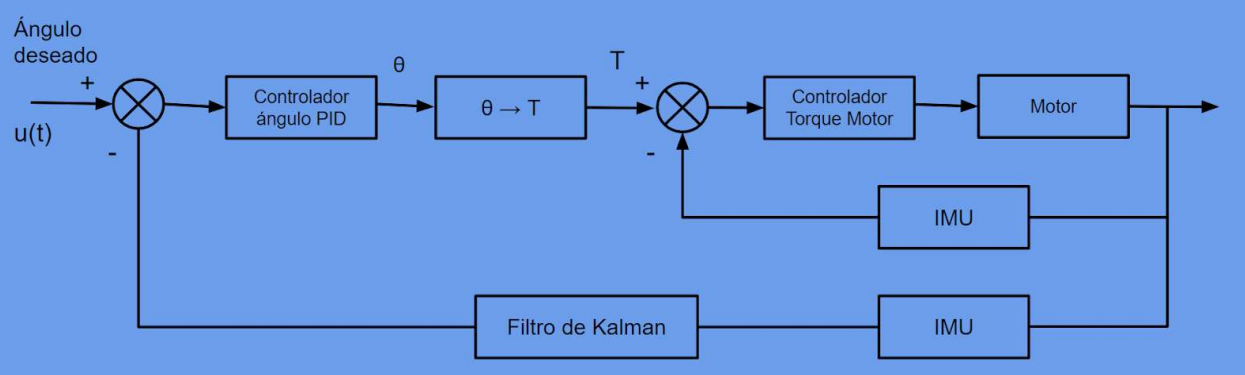
\includegraphics[width=0.8\linewidth, page=1]{Imagenes/lazo_de_control}
	\caption{Lazo de control.}
	\label{fig:control:lazo}
\end{figure}

\subsubsection{Motores FOC}
\subsubsection{Kalman Filter}


%Esquema preeliminar de control (lógica gral.) Sensores y actuadores que intervienen (no deben seleccionar o definir los componentes; solo dar una idea de qué se podría utilizar en cada caso o cual es el parámetro o variable que deberían medir).

\end{document}
